\subsection{Université de Laval}

A continuación presentamos los los gráficos resultantes de realizar una \textit{traceroute} a la página de la Université de Laval\footnote{www2.ulaval.ca.}.

\begin{figure*}
    \centering
    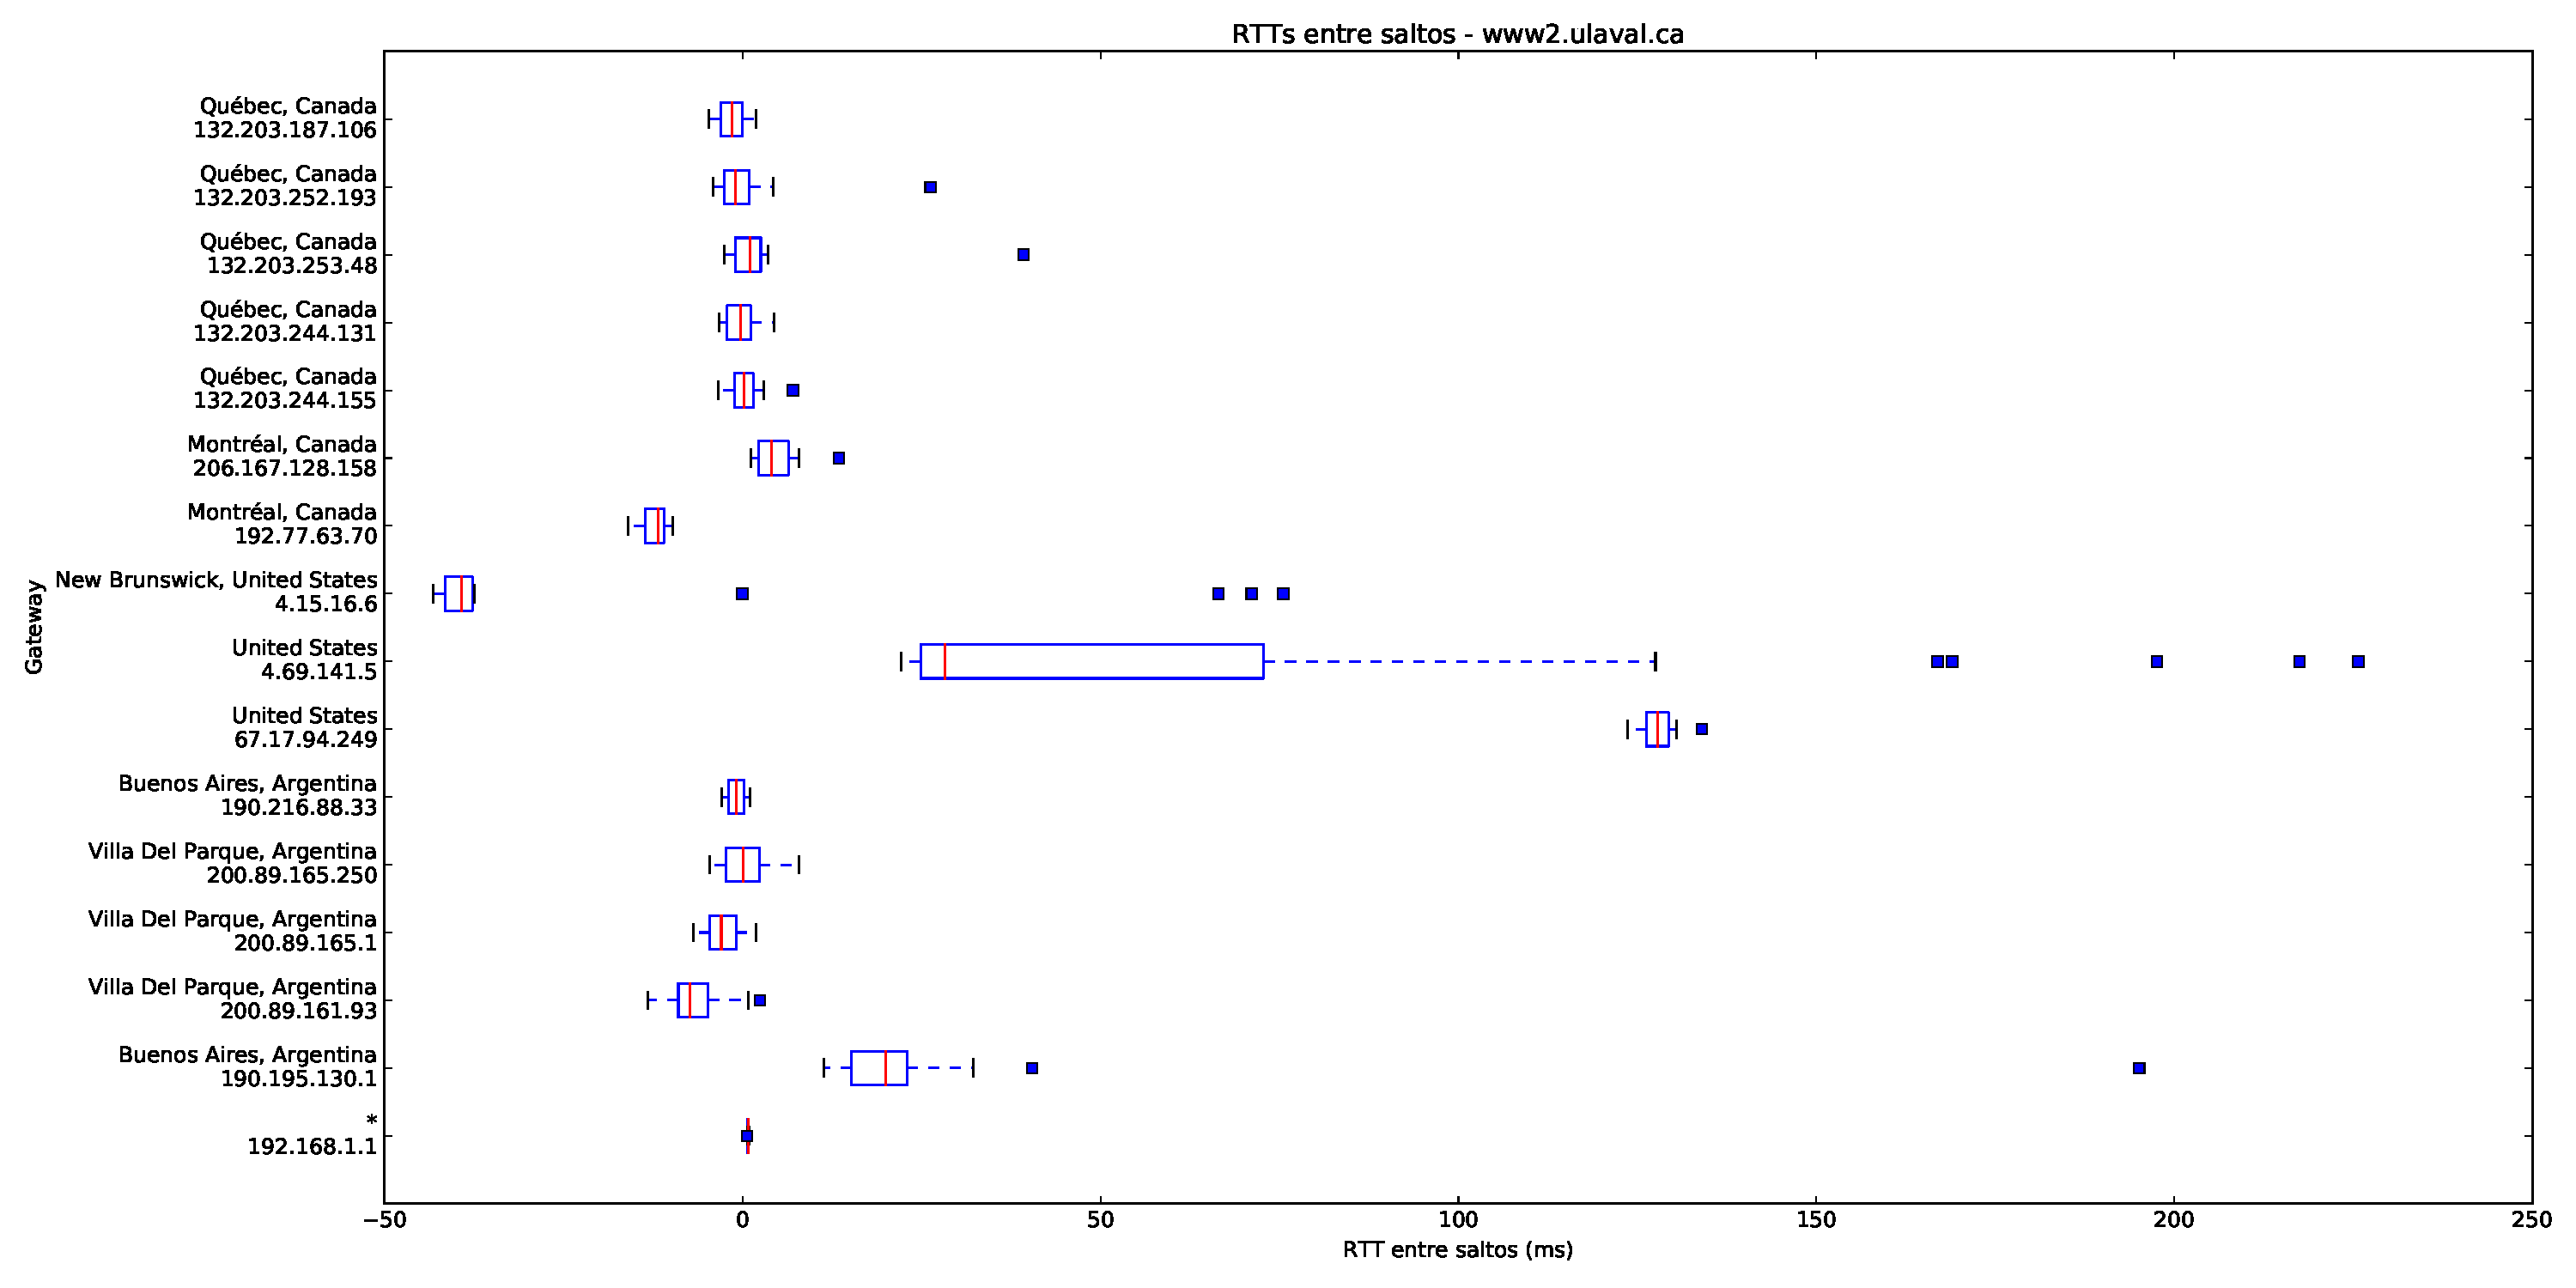
\includegraphics[width=0.9\textwidth]{img/grafico1-www2-ulaval-ca.pdf}
    \caption{RTTs entre saltos. El valor asignado al $i$-ésimo nodo corresponde al salto entre el $i$-ésimo y el $i - 1$-ésimo nodo. Para el primer nodo se utiliza simplemente su RTT.}
\end{figure*}

\begin{figure*}
    \centering
    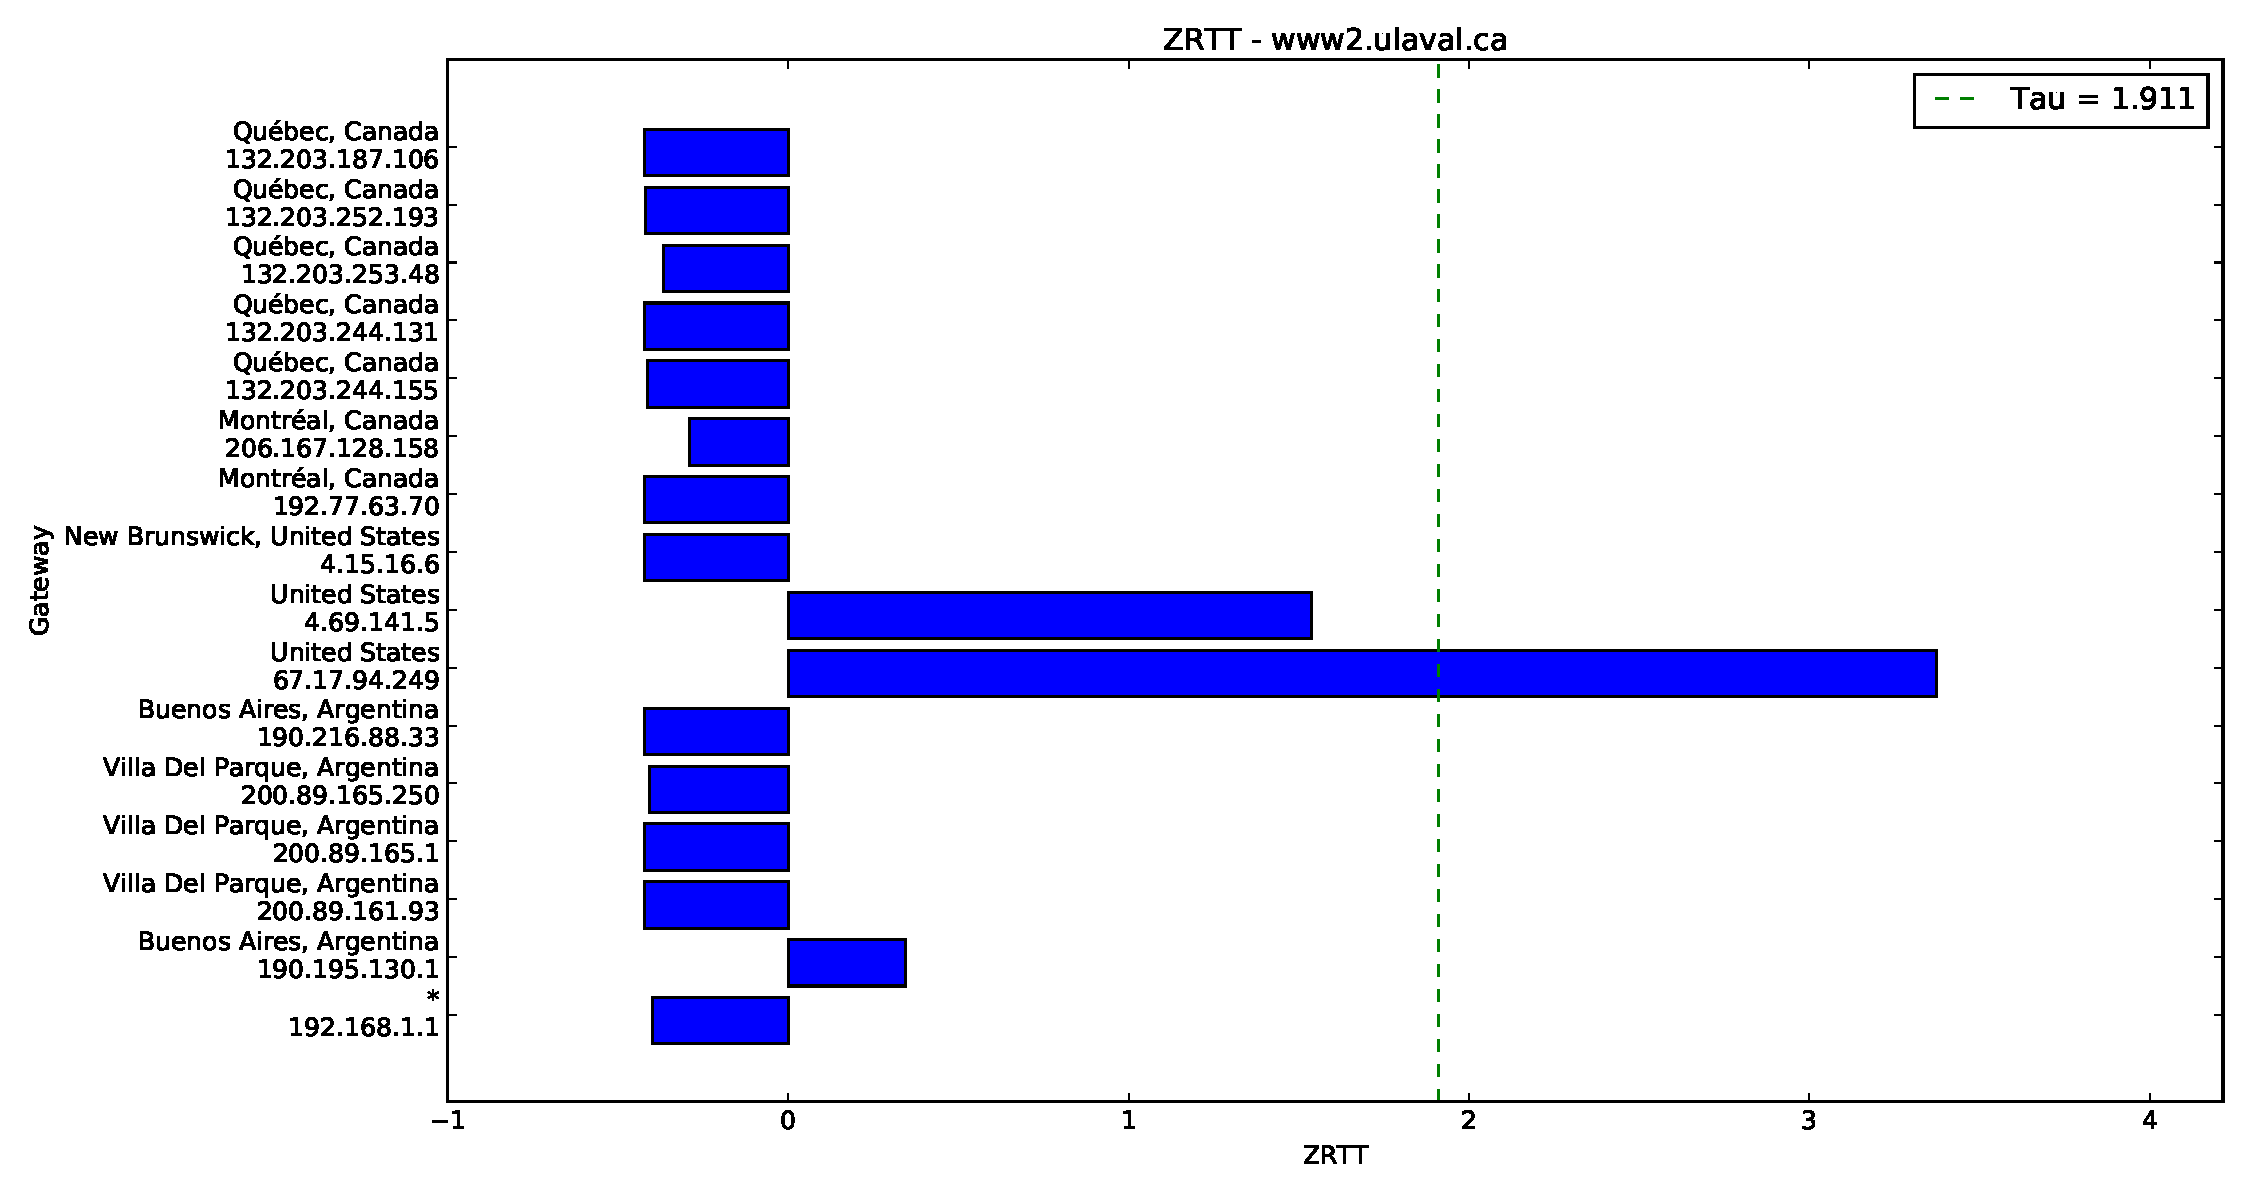
\includegraphics[width=0.9\textwidth]{img/grafico2-www2-ulaval-ca.pdf}
    \caption{ZRTTs entre saltos.}
\end{figure*}

\begin{figure*}
    \centering
    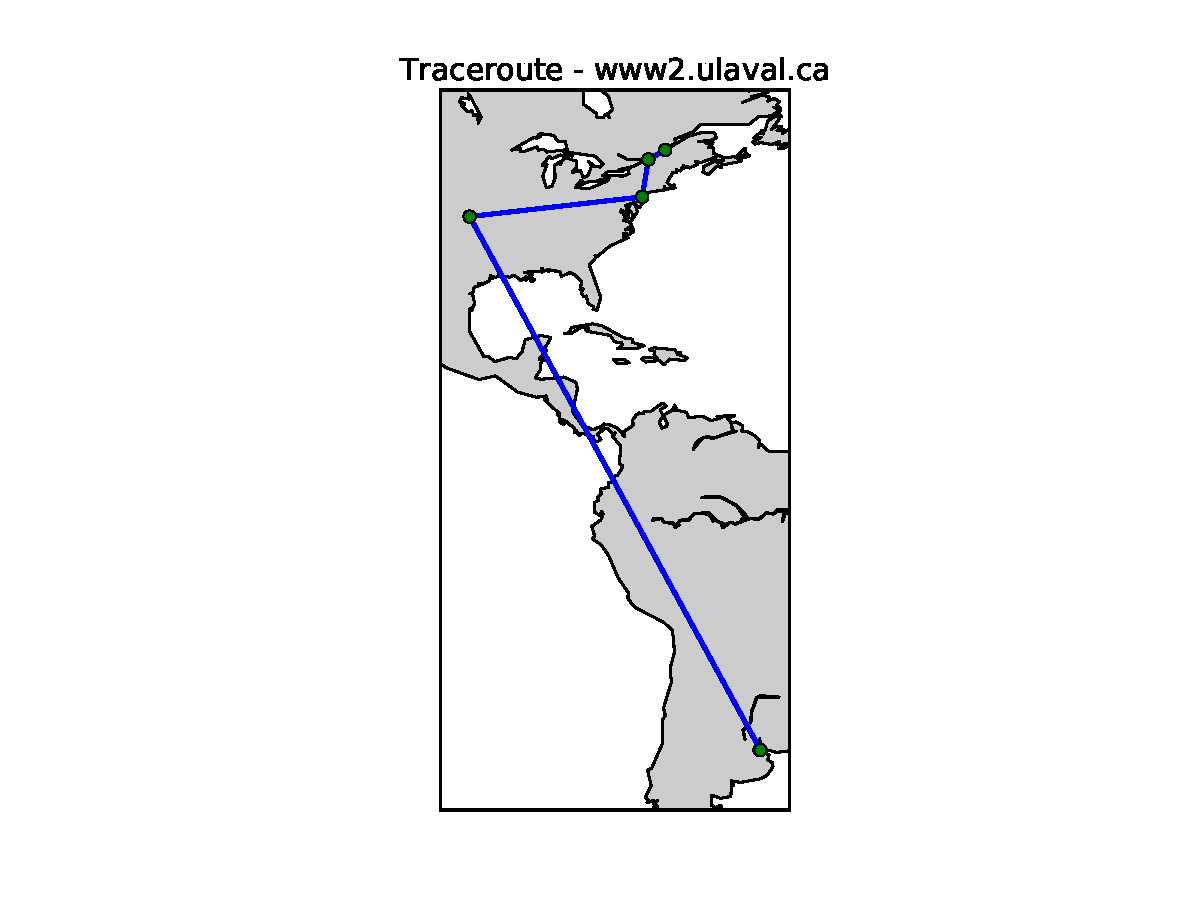
\includegraphics[width=0.9\textwidth]{img/grafico3-www2-ulaval-ca.pdf}
    \caption{Ubicación geográfica estimada de la ruta tomada.}
\end{figure*}

\par En la realización de la \textit{traceroute}, 6 de los 22 ($27.\overline{27}\%$) nodos no respondieron los \textit{Time exceeded}.

\par Sólo un salto (de 190.216.88.33 a 67.17.94.249) se presentó como \textit{outlier} según el método planteado.
De acuerdo a la estimación geográfica, este salto se da entre Buenos Aires y Estados Unidos, y efectivamente coincide con el único enlace intercontinental de la ruta.
